\chapter{Eletricidade Cerebral}

O presente capítulo apresenta uma introdução aos princípios de eletricidade cerebral, o que são ondas cerebrais e como é registrado o EEG.

\section{Correntes Elétricas e Neurônios}
%Gaspar, Alberto (2005). Física:Volume único. São Paulo: Editora Ática. 496 páginas. ISBN 9788508078837. Consultado em 12 de janeiro de 2012
A diferença de potencial elétrico (se referindo a energia necessária para deslocar uma carga elétrica (Matias e Fratezzi, 2008)) entre um material condutor gera um fluxo de cargas nomeado corrente elétrica (Creder, 1989). A intensidade deste fluxo é medida em ampère, e determinada pela quantidade de elementos carregados que atravessam o mateiral condutor. As correntes (este fluxo), podem ser contínuos ou alternados, dependendo se o sentido da corrente varia ou não; sendo a corrente contínua composta por polos, e a alternada por fases (Bhargava e Kulshreshtha, 1983). O cálculo de corrente elétrica é dado pela seguinte equação:

\begin{equation}
    I = \frac{\Delta Q }{\Delta T},
\end{equation}

onde $\Delta Q$ é a quantidade de particulas que passam em um seguimento do condutor e $\Delta T$ indica o tempo. 

Os neurônios são células responsáveis pela condução dos chamados “impulsos nervosos”, e se comportam como um “cabo eletríficado”, que é uma analogia a respeito da condução de impulsos elétricos por estas células, como apresentado no clássico estudo de Hodgkin e Huxley (1952). Os neurônios comunicam-se através de sinapses, locais onde ocorrem a transmissão destas correntes elétricas; e podem ser divididos anatomicamente em três partes: corpo celular, axônio e dendritos, apresentados na figura 2.1. A membrana celular é uma membrana semi-permeável que permite a passagem de cargas elétricas através de canais. A diferença entre a concentração destas cargas separadas pela membrana resulta em uma atuação de capacitor. Capacitores são dispositivos de polaridades diferentes em suas extremidades, capazes de armazenar cargas elétricas (Serway, 2008). Em função desta característica de separação de diferentes densidades de cargas elétricas, a membrana pode ter sua capacitância calculada pela equação 2.2
\begin{figure}
    \centering
    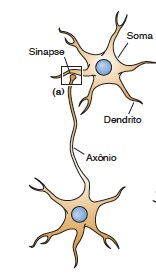
\includegraphics[width=40mm]{corpo_celular.jpg}
    \caption{Anatomia de um neurônio com destaque para área de sinapse entre neurônios. Fonte: Bear (2015)}
\end{figure}


\begin{equation}
    C = \frac{Q}{\Delta V},
\end{equation}

onde $C$ é a capacitância, $Q$ é a quantidade de carga armazenada e $\Delta V$ é a tensão elétrica, medida em farad (F). 


A resistência elétrica é outra propriedade de interesse, e se refere a capacidade de se opor a passagem de uma corrente elétrica. Esta capacidade é medida em ohms, e os canais de membrana podem se comportar como resistores a depender das condições celulares e das condições de canal, visto que estes podem estar abertos (facilitando passagem), ou não. Estes diferentes comportamentos dos componentes neuronais podem ser observados na figura 2.2.


%https://neuronaldynamics.epfl.ch/online/Ch2.S2.html#Ch2.F2
\begin{figure}
    \centering
    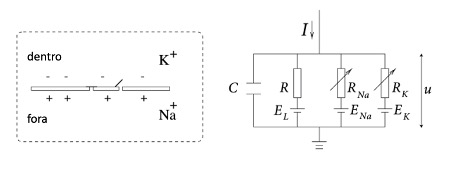
\includegraphics[width=100mm]{modeloHH.jpg}
    \caption{Esquema Modelo Hodgkin-Huxley. 
    Dentro: indicando espaço intracelular; fora: indicando espaço extracelular (imagem a esquerda). Direita: 
    C = capacitor, R = resistor, E = Baterias. Na = Sódio, K = Potássio  Fonte: Neuromal Dynamcs (2014)} 
\end{figure}

\begin{equation}
    C \frac{d u }{ d t} =  - \sum_{k} I_k (t) + I (t),
\end{equation}

onde $u$ = voltagem ao longo da membrana e $t$ = tempo. 




\section{Eletroencefalograma}

Os impulsos nervosos gerados pelos neurônios são alterações no potencial elétrico de suas membranas. 
Este sinal elétrico ocorre quando um estímulo recebido pelo neurônio é intenso o suficiente para ultrapassar seu chamado limiar de ativação.
 O conjunto de impulsos nervosos por grupos de neurônios ao longo do tempo gera campos magnéticos que podem ser captados por eletrodos 
 colocados sobre a cabeça humana (Kandel, 2000). Estes campos magnéticos foram primeiro registrados em humanos pelo psiquiatra Hans Berger 
 (Ince et al., 2021), em uma coleta representada na figura 2.4. 
 Estes registros são o resultado de potenciais de ação emitidos por células nervosas próximas ao eletrodo, 
 e permitem uma boa resolução temporal – embora não apresentem uma boa resolução espacial -  do comportamento neuronal. 



\begin{figure}[!h]
    \centering
    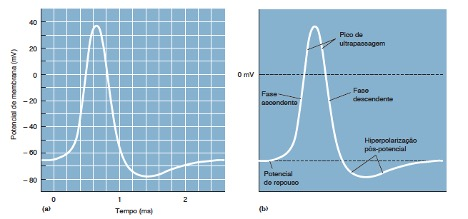
\includegraphics[width=120mm]{potencial_de_membrana_bear.jpg}
    \caption[Impulsos nervosos conduzidos em neurônios]{Resumo do potencial de ação. Fonte: Bear (2015).}.\label{fig:potencial}
    \end{figure}


  \begin{figure}[h]
    \centering
    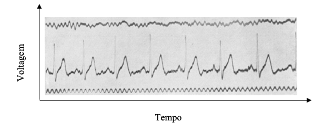
\includegraphics[width=100mm]{serie_temporal_EEG}
    \caption[]{Primeiro EEG registrado em humanos, resultado do trabalho do psiquiatra Hans Berger. Fonte: Ince et al. (2021).} 
    \end{figure}

\section{Ondas Cerebrais}
% Llinas, R. R. (2014). "Intrinsic electrical properties of mammalian neurons and CNS function: a historical perspective". Front Cell Neurosci. 8: 320. doi:10.3389/fncel.2014.00320. PMC 4219458free to read. PMID 25408634

O cérebro é capaz de gerar ondas de impulsos nervosos ritmadas. A oscilação de um único neurônio pode ser explorada na figura 2.5. As grandes oscilações são detectadas pelos eletrodos (Llinas, 2014), e classificadas de acordo com suas características. Um exemplo de agrupamento de ondas cerebrais pode ser observado na figura 2.6. 


As ondas cerebrais são caracterizadas pela \textbf{frequência, amplitude e fase} (figura 2.5). 
A amplitude mede a magnitude da oscilação de uma onda e pode ser representada pela equação

\begin{equation}
    y = A * sen (t - k) + b,
\end{equation}
onde $y$ é a função de onda (mede amplitude no instante t), $A$ é a amplitude da onda, sen representa
uma função senoidal, $t$ é o tempo, $k$ é a transalação temporal e b mede a translação de onda. 


\begin{figure}[h]
    \centering
    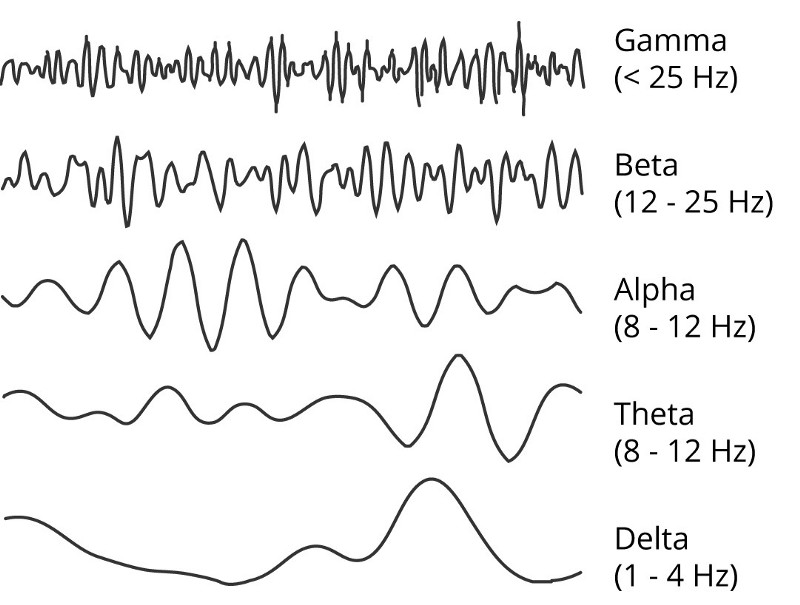
\includegraphics[width=80mm]{1_smvgacGqEOqIoKmjhzbfPw.jpeg}
    \caption[]{Ondas gamma, beta, alfa, teta e delta.} 
    \end{figure}


\subsection{Sistema Internacional 10/20 de Posicionamento de Eletrodos} 

Para garantir uma padronização a respeito da coleta de EEG, o sistema de posicionamento de eletrodos pode ser adotado. 
Em específico, sistema internacional de posicionamentos de
eletrodos para a coleta de EEG – o sistema 10/20, é uma técnica desenvolvida por Klem et al. (1999) e amplamente adotada em estudos neurocientíficos. 


O registro capturado nos eletrodos advém de uma diferença de potencial elétrico. Esta diferença pode ser em referência à
    um eletrodo colocado em uma região externa ao escalpo (como orelha), ou à uma
    voltagem média comum (Tavares, 2011).


\begin{figure}[h]
    \centering
    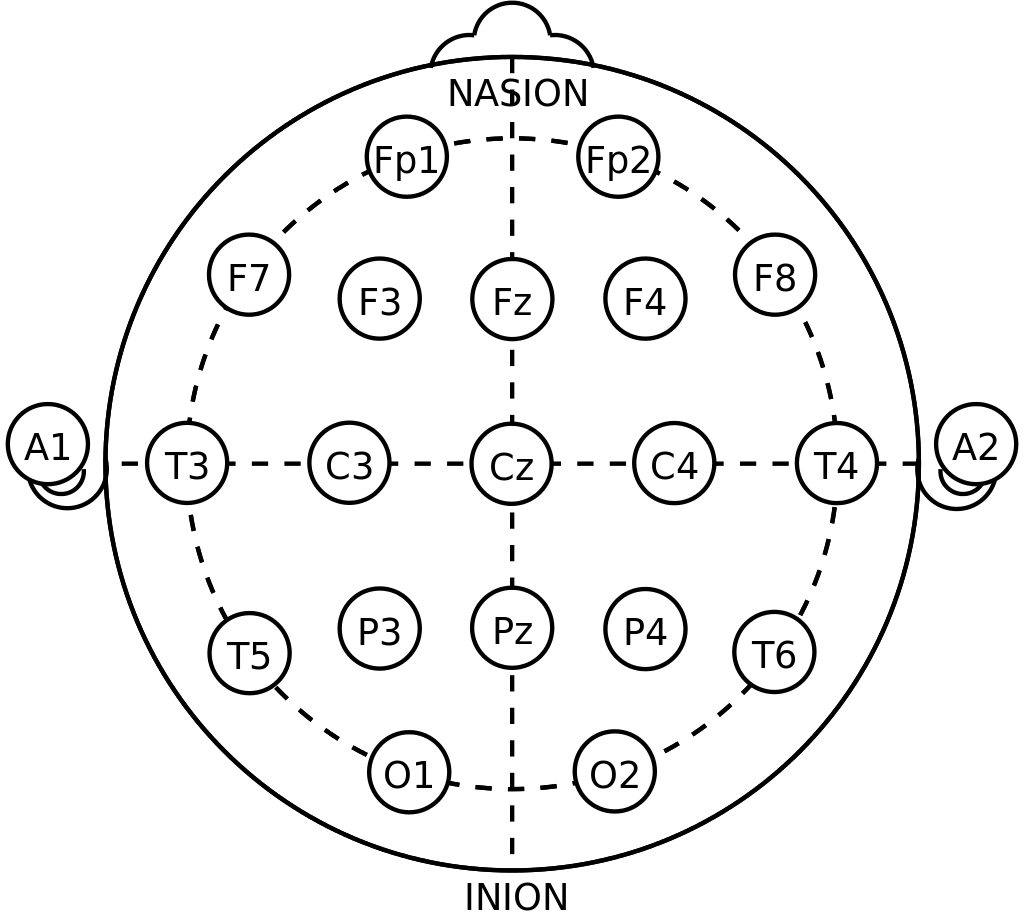
\includegraphics[width=100mm]{21_electrodes_of_International_10-20_system_for_EEG.png}
    \caption[]{Sistema Internacional 10/20 de Posicionamento de Eletrodos. Em destaque:
    Posição do eletrodo de coleta passiva do MindWave Mobile 2. A = Ear lobe, AF = anterior
    frontal, C = central, CP = centroparietal, F = frontal, FC = frontocentral, FT =
    frontotemporal, N = nasion, O = occipital, P = parietal, PO = parietooccipital, T = temporal.
    
    Klem et al. (1999).} 
    \end{figure}
    
    
        
\subsection{Tipos de Eletrodos para Captura de EEG}

Existem diferentes tipos de eletrodos para a captura de EEG, e uma descrição deles pode ser encontrada no quadro 2.1. 
Cada tipo de equipamento de coleta irá ter seu tipo de eletrodo. No caso de equipamentos de coleta de EEG comerciais, 
é comum a presença do eletrodo do tipo seco – que requer menos preparo, dispensando a aplicação de gel (Brain Support Inc., 2019).  
É notável também que com o 
    desenvolvimento da capacidade computacional, novos recursos e métodos 
    para a análise destes dados vem sendo benéficos à construção do conhecimento 
    científico, agora também contando com o desenvolvimento de algoritmos de aprendizado
     de máquina, aprendizado profundo e inteligência artificial. 

     \begin{quadro}
        \caption{Tipos de Eletrodos para coleta de EEG (adaptado de Brain Support Inc. (2019)):}\label{quadro:exemplo}
        \begin{center}
        \scalefont{0.905}
        \begin{tabular}{|l|l|}
        \hline
        \hfill Tipo de Eletrodo\hfill\hspace{1mm} & \hfill Descrição\hfill\hspace{1mm}\\
        \hline
        Passivo &  \hspace{-06pt}\begin{tabular}{l}Geralmente feitos de prata, contam com a aplicação 
            de gel condutor \\
        para reduzir a perda de informação antes de serem colocados \\ na cabeça do participante.\end{tabular}\\
        \hline
        Ativo & \hspace{-06pt}\begin{tabular}{l}Geralmente feitos em prata, permitem o registro de \\
            variações de voltagem com redução de ruído do ambiente \\
            através de um circuito integrado aos eletrodos, com \\
            conversores de impedância.\end{tabular}\\
        \hline
        Seco & \hspace{-06pt}\begin{tabular}{l}Não necessita da aplicação de gel 
            para melhora da coleta do sinal.\end{tabular}\\
        \hline
        \end{tabular}
        \scalefont{1.4184}
        \end{center}
        \vspace{-12pt}
        Fonte: Brain Support Inc. (2019).\\
        \end{quadro}
        
  

    % Please add the following required packages to your document preamble:
% Please add the following required packages to your document preamble:
% \usepackage{graphicx}



%\subsection{Potenciais Relacionados a Eventos}


